% Options for packages loaded elsewhere
\PassOptionsToPackage{unicode}{hyperref}
\PassOptionsToPackage{hyphens}{url}
\PassOptionsToPackage{dvipsnames,svgnames,x11names}{xcolor}
%
\documentclass[
  letterpaper,
  DIV=11,
  numbers=noendperiod]{scrartcl}

\usepackage{amsmath,amssymb}
\usepackage{iftex}
\ifPDFTeX
  \usepackage[T1]{fontenc}
  \usepackage[utf8]{inputenc}
  \usepackage{textcomp} % provide euro and other symbols
\else % if luatex or xetex
  \usepackage{unicode-math}
  \defaultfontfeatures{Scale=MatchLowercase}
  \defaultfontfeatures[\rmfamily]{Ligatures=TeX,Scale=1}
\fi
\usepackage{lmodern}
\ifPDFTeX\else  
    % xetex/luatex font selection
\fi
% Use upquote if available, for straight quotes in verbatim environments
\IfFileExists{upquote.sty}{\usepackage{upquote}}{}
\IfFileExists{microtype.sty}{% use microtype if available
  \usepackage[]{microtype}
  \UseMicrotypeSet[protrusion]{basicmath} % disable protrusion for tt fonts
}{}
\makeatletter
\@ifundefined{KOMAClassName}{% if non-KOMA class
  \IfFileExists{parskip.sty}{%
    \usepackage{parskip}
  }{% else
    \setlength{\parindent}{0pt}
    \setlength{\parskip}{6pt plus 2pt minus 1pt}}
}{% if KOMA class
  \KOMAoptions{parskip=half}}
\makeatother
\usepackage{xcolor}
\setlength{\emergencystretch}{3em} % prevent overfull lines
\setcounter{secnumdepth}{-\maxdimen} % remove section numbering
% Make \paragraph and \subparagraph free-standing
\ifx\paragraph\undefined\else
  \let\oldparagraph\paragraph
  \renewcommand{\paragraph}[1]{\oldparagraph{#1}\mbox{}}
\fi
\ifx\subparagraph\undefined\else
  \let\oldsubparagraph\subparagraph
  \renewcommand{\subparagraph}[1]{\oldsubparagraph{#1}\mbox{}}
\fi

\usepackage{color}
\usepackage{fancyvrb}
\newcommand{\VerbBar}{|}
\newcommand{\VERB}{\Verb[commandchars=\\\{\}]}
\DefineVerbatimEnvironment{Highlighting}{Verbatim}{commandchars=\\\{\}}
% Add ',fontsize=\small' for more characters per line
\usepackage{framed}
\definecolor{shadecolor}{RGB}{241,243,245}
\newenvironment{Shaded}{\begin{snugshade}}{\end{snugshade}}
\newcommand{\AlertTok}[1]{\textcolor[rgb]{0.68,0.00,0.00}{#1}}
\newcommand{\AnnotationTok}[1]{\textcolor[rgb]{0.37,0.37,0.37}{#1}}
\newcommand{\AttributeTok}[1]{\textcolor[rgb]{0.40,0.45,0.13}{#1}}
\newcommand{\BaseNTok}[1]{\textcolor[rgb]{0.68,0.00,0.00}{#1}}
\newcommand{\BuiltInTok}[1]{\textcolor[rgb]{0.00,0.23,0.31}{#1}}
\newcommand{\CharTok}[1]{\textcolor[rgb]{0.13,0.47,0.30}{#1}}
\newcommand{\CommentTok}[1]{\textcolor[rgb]{0.37,0.37,0.37}{#1}}
\newcommand{\CommentVarTok}[1]{\textcolor[rgb]{0.37,0.37,0.37}{\textit{#1}}}
\newcommand{\ConstantTok}[1]{\textcolor[rgb]{0.56,0.35,0.01}{#1}}
\newcommand{\ControlFlowTok}[1]{\textcolor[rgb]{0.00,0.23,0.31}{#1}}
\newcommand{\DataTypeTok}[1]{\textcolor[rgb]{0.68,0.00,0.00}{#1}}
\newcommand{\DecValTok}[1]{\textcolor[rgb]{0.68,0.00,0.00}{#1}}
\newcommand{\DocumentationTok}[1]{\textcolor[rgb]{0.37,0.37,0.37}{\textit{#1}}}
\newcommand{\ErrorTok}[1]{\textcolor[rgb]{0.68,0.00,0.00}{#1}}
\newcommand{\ExtensionTok}[1]{\textcolor[rgb]{0.00,0.23,0.31}{#1}}
\newcommand{\FloatTok}[1]{\textcolor[rgb]{0.68,0.00,0.00}{#1}}
\newcommand{\FunctionTok}[1]{\textcolor[rgb]{0.28,0.35,0.67}{#1}}
\newcommand{\ImportTok}[1]{\textcolor[rgb]{0.00,0.46,0.62}{#1}}
\newcommand{\InformationTok}[1]{\textcolor[rgb]{0.37,0.37,0.37}{#1}}
\newcommand{\KeywordTok}[1]{\textcolor[rgb]{0.00,0.23,0.31}{#1}}
\newcommand{\NormalTok}[1]{\textcolor[rgb]{0.00,0.23,0.31}{#1}}
\newcommand{\OperatorTok}[1]{\textcolor[rgb]{0.37,0.37,0.37}{#1}}
\newcommand{\OtherTok}[1]{\textcolor[rgb]{0.00,0.23,0.31}{#1}}
\newcommand{\PreprocessorTok}[1]{\textcolor[rgb]{0.68,0.00,0.00}{#1}}
\newcommand{\RegionMarkerTok}[1]{\textcolor[rgb]{0.00,0.23,0.31}{#1}}
\newcommand{\SpecialCharTok}[1]{\textcolor[rgb]{0.37,0.37,0.37}{#1}}
\newcommand{\SpecialStringTok}[1]{\textcolor[rgb]{0.13,0.47,0.30}{#1}}
\newcommand{\StringTok}[1]{\textcolor[rgb]{0.13,0.47,0.30}{#1}}
\newcommand{\VariableTok}[1]{\textcolor[rgb]{0.07,0.07,0.07}{#1}}
\newcommand{\VerbatimStringTok}[1]{\textcolor[rgb]{0.13,0.47,0.30}{#1}}
\newcommand{\WarningTok}[1]{\textcolor[rgb]{0.37,0.37,0.37}{\textit{#1}}}

\providecommand{\tightlist}{%
  \setlength{\itemsep}{0pt}\setlength{\parskip}{0pt}}\usepackage{longtable,booktabs,array}
\usepackage{calc} % for calculating minipage widths
% Correct order of tables after \paragraph or \subparagraph
\usepackage{etoolbox}
\makeatletter
\patchcmd\longtable{\par}{\if@noskipsec\mbox{}\fi\par}{}{}
\makeatother
% Allow footnotes in longtable head/foot
\IfFileExists{footnotehyper.sty}{\usepackage{footnotehyper}}{\usepackage{footnote}}
\makesavenoteenv{longtable}
\usepackage{graphicx}
\makeatletter
\def\maxwidth{\ifdim\Gin@nat@width>\linewidth\linewidth\else\Gin@nat@width\fi}
\def\maxheight{\ifdim\Gin@nat@height>\textheight\textheight\else\Gin@nat@height\fi}
\makeatother
% Scale images if necessary, so that they will not overflow the page
% margins by default, and it is still possible to overwrite the defaults
% using explicit options in \includegraphics[width, height, ...]{}
\setkeys{Gin}{width=\maxwidth,height=\maxheight,keepaspectratio}
% Set default figure placement to htbp
\makeatletter
\def\fps@figure{htbp}
\makeatother

\usepackage{float}
\usepackage{tabularray}
\usepackage[normalem]{ulem}
\usepackage{graphicx}
\UseTblrLibrary{booktabs}
\UseTblrLibrary{siunitx}
\NewTableCommand{\tinytableDefineColor}[3]{\definecolor{#1}{#2}{#3}}
\newcommand{\tinytableTabularrayUnderline}[1]{\underline{#1}}
\newcommand{\tinytableTabularrayStrikeout}[1]{\sout{#1}}
\KOMAoption{captions}{tableheading}
\makeatletter
\@ifpackageloaded{caption}{}{\usepackage{caption}}
\AtBeginDocument{%
\ifdefined\contentsname
  \renewcommand*\contentsname{Table of contents}
\else
  \newcommand\contentsname{Table of contents}
\fi
\ifdefined\listfigurename
  \renewcommand*\listfigurename{List of Figures}
\else
  \newcommand\listfigurename{List of Figures}
\fi
\ifdefined\listtablename
  \renewcommand*\listtablename{List of Tables}
\else
  \newcommand\listtablename{List of Tables}
\fi
\ifdefined\figurename
  \renewcommand*\figurename{Figure}
\else
  \newcommand\figurename{Figure}
\fi
\ifdefined\tablename
  \renewcommand*\tablename{Table}
\else
  \newcommand\tablename{Table}
\fi
}
\@ifpackageloaded{float}{}{\usepackage{float}}
\floatstyle{ruled}
\@ifundefined{c@chapter}{\newfloat{codelisting}{h}{lop}}{\newfloat{codelisting}{h}{lop}[chapter]}
\floatname{codelisting}{Listing}
\newcommand*\listoflistings{\listof{codelisting}{List of Listings}}
\makeatother
\makeatletter
\makeatother
\makeatletter
\@ifpackageloaded{caption}{}{\usepackage{caption}}
\@ifpackageloaded{subcaption}{}{\usepackage{subcaption}}
\makeatother
\ifLuaTeX
  \usepackage{selnolig}  % disable illegal ligatures
\fi
\usepackage{bookmark}

\IfFileExists{xurl.sty}{\usepackage{xurl}}{} % add URL line breaks if available
\urlstyle{same} % disable monospaced font for URLs
\hypersetup{
  pdftitle={401-2\_Homework2},
  pdfauthor={Cat Dang Ton},
  colorlinks=true,
  linkcolor={blue},
  filecolor={Maroon},
  citecolor={Blue},
  urlcolor={Blue},
  pdfcreator={LaTeX via pandoc}}

\title{401-2\_Homework2}
\author{Cat Dang Ton}
\date{2024-04-14}

\begin{document}
\maketitle

sigtop export-messages messages sigtop export-attachments attachments

\subsection{Question 1}\label{question-1}

I am still using data from the 2022 Health and Retirement Survey. The
sample consists of respondents to the survey's subsection on Widowhood
and Divorce, who experienced the death of a spouse between 2020 and
2022.

Dependent variable: whether or not the widow had to sell assets,
withdraw money that normally would not be touched, get help from a
relative, or from a church or other institution, or do anything else
special to find the money to cover the deceased spouse's death expenses
(funeral expenses, legal fees, expenses for any illness that led to
death). (Yes = 1, No = 0).

Independent variables:

\begin{enumerate}
\def\labelenumi{\arabic{enumi}.}
\tightlist
\item
  Whether the living spouse is US-born or foreign born (US-born = 1,
  foreign-born = 0)
\item
  Total death expenses that are NOT covered by insurance or the deceased
  spouse's estate (Exact dollar amounts, or if not available, the
  midpoint of approximated estimates)
\item
  The widow's level of education (note: widow's income calculations are
  forthcoming. Education is a stand-in for now.)
\end{enumerate}

\subsubsection{A.}\label{a.}

\begin{Shaded}
\begin{Highlighting}[]
\CommentTok{\# Convert dependent variable and continuous variable to numeric so the model takes it}
\NormalTok{df}\SpecialCharTok{$}\NormalTok{deathexpense\_special }\OtherTok{\textless{}{-}} \FunctionTok{as.numeric}\NormalTok{(df}\SpecialCharTok{$}\NormalTok{deathexpense\_special)}
\NormalTok{df}\SpecialCharTok{$}\NormalTok{deathexpense\_usd }\OtherTok{\textless{}{-}} \FunctionTok{as.numeric}\NormalTok{(df}\SpecialCharTok{$}\NormalTok{deathexpense\_usd)}
\CommentTok{\# convert unit of analysis to thousands of dollars}
\NormalTok{df}\SpecialCharTok{$}\NormalTok{deathexpense\_1k }\OtherTok{\textless{}{-}}\NormalTok{ df}\SpecialCharTok{$}\NormalTok{deathexpense\_usd}\SpecialCharTok{/}\DecValTok{1000} 
\CommentTok{\# run model}
\NormalTok{model }\OtherTok{\textless{}{-}} \FunctionTok{lm\_robust}\NormalTok{(deathexpense\_special }\SpecialCharTok{\textasciitilde{}}\NormalTok{ usborn }\SpecialCharTok{+}\NormalTok{ deathexpense\_1k }\SpecialCharTok{+}\NormalTok{ degree, }\AttributeTok{data =}\NormalTok{ df)}

\FunctionTok{modelsummary}\NormalTok{(model)}
\end{Highlighting}
\end{Shaded}

\begin{table}
\centering
\begin{tblr}[         %% tabularray outer open
]                     %% tabularray outer close
{                     %% tabularray inner open
colspec={Q[]Q[]},
column{1}={halign=l,},
column{2}={halign=c,},
hline{18}={1,2}{solid, 0.05em, black},
}                     %% tabularray inner close
\toprule
& (1) \\ \midrule %% TinyTableHeader
(Intercept)                       & \num{0.363}   \\
& (\num{0.074}) \\
usbornus-born                     & \num{-0.127}  \\
& (\num{0.054}) \\
deathexpense\_1k                 & \num{0.006}   \\
& (\num{0.004}) \\
degreeDegree unknown/Some College & \num{0.037}   \\
& (\num{0.098}) \\
degreeGED                         & \num{-0.046}  \\
& (\num{0.078}) \\
degreeHigh school diploma         & \num{-0.071}  \\
& (\num{0.046}) \\
degreeNo degree                   & \num{-0.028}  \\
& (\num{0.057}) \\
degreePostgraduate degree         & \num{-0.066}  \\
& (\num{0.073}) \\
Num.Obs.                          & \num{741}     \\
R2                                & \num{0.031}   \\
R2 Adj.                           & \num{0.022}   \\
AIC                               & \num{853.5}   \\
BIC                               & \num{894.9}   \\
RMSE                              & \num{0.43}    \\
\bottomrule
\end{tblr}
\end{table}

Reference category: College-educated foreign-born person, who has no
death expenses beyond what is covered by insurance or by their deceased
spouse's estate.

The number of cases in the model is 741.

The slope for US-born respondents suggests that, after controlling for
the amount final expenses not covered by insurance and for their level
of education, a widow's US-born status renders them 23\% less likely to
have to resort to special means to finance final expenses, compared to
foreign-born widows.

\subsubsection{B.}\label{b.}

\begin{Shaded}
\begin{Highlighting}[]
\CommentTok{\# Generate predicted values}
\NormalTok{df}\SpecialCharTok{$}\NormalTok{predicted\_prob }\OtherTok{\textless{}{-}} \FunctionTok{predict}\NormalTok{(model, }\AttributeTok{newdata =}\NormalTok{ df)}

\CommentTok{\# Create a scatter plot of the predicted probabilities}
\FunctionTok{ggplot}\NormalTok{(df, }\FunctionTok{aes}\NormalTok{(}\AttributeTok{x =}\NormalTok{ usborn, }\AttributeTok{y =}\NormalTok{ predicted\_prob)) }\SpecialCharTok{+}
  \FunctionTok{geom\_point}\NormalTok{() }\SpecialCharTok{+}
  \FunctionTok{labs}\NormalTok{(}\AttributeTok{x =} \StringTok{"US Born"}\NormalTok{, }\AttributeTok{y =} \StringTok{"Predicted Probability of Special Death Expenses"}\NormalTok{) }\SpecialCharTok{+}
  \FunctionTok{theme\_minimal}\NormalTok{()}
\end{Highlighting}
\end{Shaded}

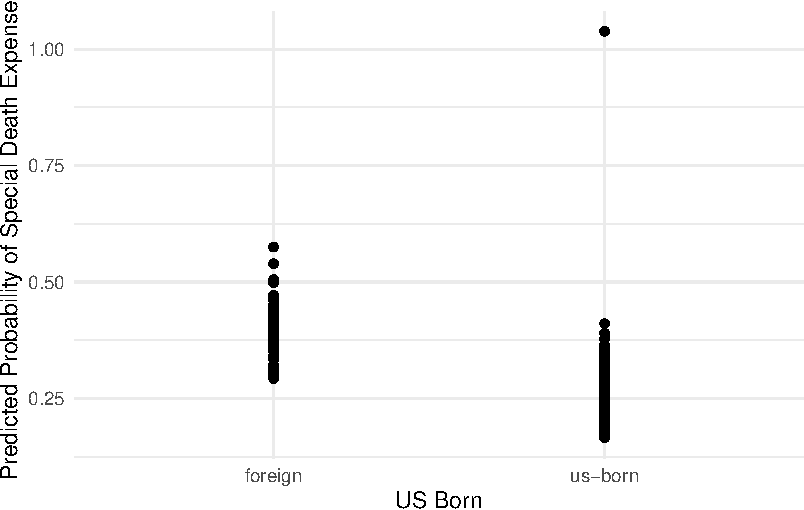
\includegraphics{homework2_Ton_files/figure-pdf/predicted_values_ols_plot-1.pdf}

\subsubsection{C.}\label{c.}

\begin{Shaded}
\begin{Highlighting}[]
\CommentTok{\# Estimate a logistic regression model}
\NormalTok{model\_logit }\OtherTok{\textless{}{-}} \FunctionTok{glm}\NormalTok{(deathexpense\_special }\SpecialCharTok{\textasciitilde{}}\NormalTok{ usborn }\SpecialCharTok{+}\NormalTok{ degree }\SpecialCharTok{+}\NormalTok{ deathexpense\_1k, }
  \AttributeTok{data =}\NormalTok{ df, }
  \AttributeTok{family =} \FunctionTok{binomial}\NormalTok{(}\AttributeTok{link =} \StringTok{"logit"}\NormalTok{)) }\CommentTok{\#specify that we want logistic regression(link = "logit")) }
\FunctionTok{modelsummary}\NormalTok{(model\_logit) }\CommentTok{\# print logit regression estimates}
\end{Highlighting}
\end{Shaded}

\begin{table}
\centering
\begin{tblr}[         %% tabularray outer open
]                     %% tabularray outer close
{                     %% tabularray inner open
colspec={Q[]Q[]},
column{1}={halign=l,},
column{2}={halign=c,},
hline{18}={1,2}{solid, 0.05em, black},
}                     %% tabularray inner close
\toprule
& (1) \\ \midrule %% TinyTableHeader
(Intercept)                       & \num{-0.590}   \\
& (\num{0.313})  \\
usbornus-born                     & \num{-0.601}   \\
& (\num{0.240})  \\
degreeDegree unknown/Some College & \num{0.176}    \\
& (\num{0.457})  \\
degreeGED                         & \num{-0.252}   \\
& (\num{0.436})  \\
degreeHigh school diploma         & \num{-0.384}   \\
& (\num{0.235})  \\
degreeNo degree                   & \num{-0.147}   \\
& (\num{0.291})  \\
degreePostgraduate degree         & \num{-0.369}   \\
& (\num{0.402})  \\
deathexpense\_1k                 & \num{0.032}    \\
& (\num{0.012})  \\
Num.Obs.                          & \num{741}      \\
AIC                               & \num{824.7}    \\
BIC                               & \num{861.5}    \\
Log.Lik.                          & \num{-404.329} \\
F                                 & \num{2.910}    \\
RMSE                              & \num{0.42}     \\
\bottomrule
\end{tblr}
\end{table}

\begin{Shaded}
\begin{Highlighting}[]
\CommentTok{\# Calculate and print odds ratios}
\FunctionTok{rbind}\NormalTok{(}\FunctionTok{coef}\NormalTok{(model\_logit), }\CommentTok{\# get coefficients}
  \FunctionTok{exp}\NormalTok{(}\FunctionTok{coef}\NormalTok{(model\_logit))) }\CommentTok{\# get odds ratios}
\end{Highlighting}
\end{Shaded}

\begin{verbatim}
     (Intercept) usbornus-born degreeDegree unknown/Some College  degreeGED
[1,]  -0.5898708    -0.6005425                         0.1762282 -0.2516803
[2,]   0.5543989     0.5485140                         1.1927102  0.7774932
     degreeHigh school diploma degreeNo degree degreePostgraduate degree
[1,]                -0.3842166      -0.1468196                -0.3689075
[2,]                 0.6809839       0.8634497                 0.6914893
     deathexpense_1k
[1,]      0.03173747
[2,]      1.03224647
\end{verbatim}

Reference category: College-educated foreign-born person, who has no
death expenses beyond what is covered by insurance or by their deceased
spouse's estate.

US-born: the logged odds of resorting to special means to finance death
expenses are lower by 0.60 for US-born widows than for foreign-born
widows, holding all other variables constant. The odds of resorting to
special means to finance death expenses are 46\% lower for US-born
widows than for foreign-born widows.

Degree: Compared to those with a college degree, the logged odds of
resorting to special means to finance death expenses are lower for those
with no degree, those with a GED, a high school diploma, or a
postgraduate degree. The odds of resorting to special means to finance
death expenses are 14\% lower for those with no degree, 23\% lower for
those with a GED, 32\% lower for those with a high school diploma, 31\%
lower for those with a postgraduate degree, and 19\% higher for those
who enrolled in college without obtaining a degree.

Death expenses: the logged odds of resorting to special means to finance
death expenses increase by 0.03 for each thousand-dollar increase in
such expenses. Each additional thousand dollars in death expenses not
covered by insurance increases the odds of resorting to special means of
financing them by 3\%.

\subsubsection{D.}\label{d.}

\begin{Shaded}
\begin{Highlighting}[]
\CommentTok{\# Average Marginal Effects is:}
\CommentTok{\# The average of all observation{-}specific marginal effects}
\FunctionTok{avg\_slopes}\NormalTok{(model\_logit)}
\end{Highlighting}
\end{Shaded}

\begin{verbatim}

            Term                                     Contrast Estimate
 deathexpense_1k dY/dX                                         0.00574
 degree          Degree unknown/Some College - College degree  0.03689
 degree          GED - College degree                         -0.04832
 degree          High school diploma - College degree         -0.07153
 degree          No degree - College degree                   -0.02884
 degree          Postgraduate degree - College degree         -0.06893
 usborn          us-born - foreign                            -0.12048
 Std. Error      z Pr(>|z|)   S   2.5 %   97.5 %
    0.00216  2.654  0.00795 7.0  0.0015  0.00997
    0.09755  0.378  0.70530 0.5 -0.1543  0.22809
    0.08102 -0.596  0.55095 0.9 -0.2071  0.11048
    0.04555 -1.570  0.11634 3.1 -0.1608  0.01775
    0.05697 -0.506  0.61261 0.7 -0.1405  0.08281
    0.07196 -0.958  0.33811 1.6 -0.2100  0.07211
    0.05217 -2.309  0.02092 5.6 -0.2227 -0.01823

Columns: term, contrast, estimate, std.error, statistic, p.value, s.value, conf.low, conf.high 
Type:  response 
\end{verbatim}

Among the variables in the model, it seems the most important predictor
of whether or not a widow turns to special means to finance their
deceased spouse's final expenses is the widow's US-born status because
the estimate is statistically significant at 0.05, the coefficient
estimate for usborn has the largest absolute value among the
coefficients, the confidence interval does not include 0, and the
standard error is relatively small.

\subsubsection{E.}\label{e.}

\begin{Shaded}
\begin{Highlighting}[]
\CommentTok{\# 1. Graph the probability of the outcome for values of one of the independent variables, }
\CommentTok{\# holding the other variables at their mean or mode.}
\CommentTok{\# Also known as the default setting of plot\_predictions.}
\CommentTok{\# condition = independent variable of interest.}
\CommentTok{\# if condition var = continuous, plot\_predictions plots the mean.}
\FunctionTok{plot\_predictions}\NormalTok{(model\_logit, }\AttributeTok{condition =} \StringTok{"deathexpense\_1k"}\NormalTok{) }\CommentTok{\# continuous indep. var.}
\end{Highlighting}
\end{Shaded}

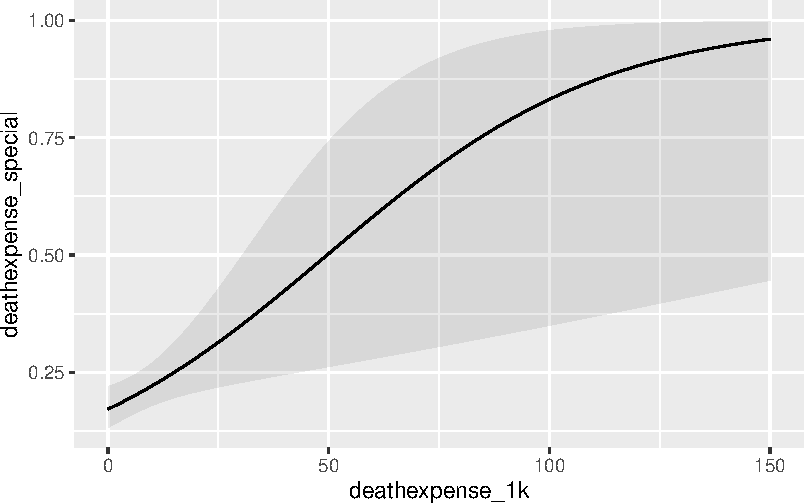
\includegraphics{homework2_Ton_files/figure-pdf/unnamed-chunk-4-1.pdf}

\begin{Shaded}
\begin{Highlighting}[]
\CommentTok{\# 2. Plot average predictions }
\CommentTok{\# graph average predictions based on letting controls retain original values,}
\CommentTok{\# but changing X rather than holding other variables at mean/mode.}
\CommentTok{\# this is known as a "counterfactual" grid type in plot\_predictions()}
\FunctionTok{plot\_predictions}\NormalTok{(model\_logit, }\AttributeTok{by =} \StringTok{"deathexpense\_1k"}\NormalTok{, }\AttributeTok{newdata =} \FunctionTok{datagrid}\NormalTok{(}\AttributeTok{deathexpense\_1k =} \DecValTok{0}\SpecialCharTok{:}\DecValTok{700}\NormalTok{, }\AttributeTok{grid\_type =} \StringTok{"counterfactual"}\NormalTok{), }\AttributeTok{type =} \StringTok{"response"}\NormalTok{)}
\end{Highlighting}
\end{Shaded}

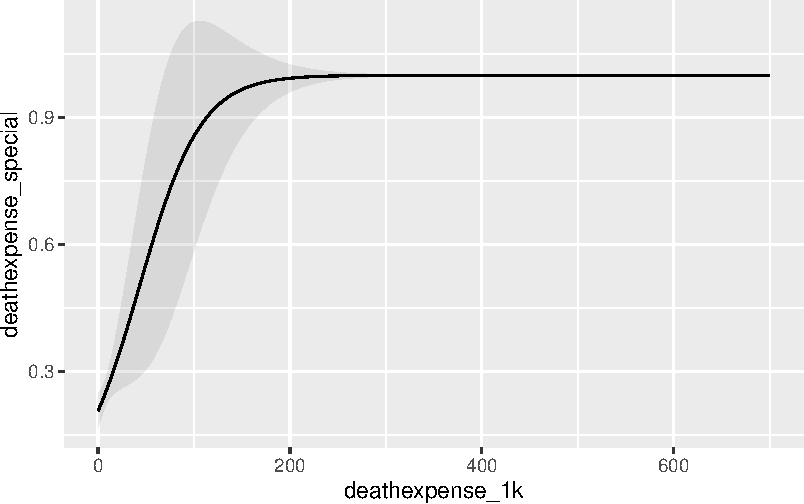
\includegraphics{homework2_Ton_files/figure-pdf/unnamed-chunk-4-2.pdf}

\subsection{Question 2}\label{question-2}

\subsubsection{A.}\label{a.-1}

Outcome variable: whether or not the speech contains populist claims,
based on an iteratively defined dictionary of populist terms. It is a
binomial variable with 0 and 1 values.

Main independent variables:

\begin{itemize}
\tightlist
\item
  Party (Republican or Democratic),
\item
  party incumbency,
\item
  prior office,
\item
  political career length,
\item
  phase of campaign in relation to election day,
\item
  interaction term between field position and campaign duration (?)
  (from Hypothesis 6; but regression table 2 did not have an interaction
  term?)
\item
  Geographic region
\end{itemize}

\subsubsection{B.}\label{b.-1}

The odds ratio of an incumbent's speech being populist is 0.279, which
means that for every political speech from an incumbent party member
that contains a populist claim, there would be nearly 4 speeches from
challengers containing a populist claim. Incumbents are thus less likely
to make populist claims than challengers.

Controls were included for length of speech, because the longer the
speech, the more likely it is to contain a populist claim.

\subsubsection{C.}\label{c.-1}

For a baseline probability of 0.3, the effect of being part of the
incumbent party on the proability of using populist rhetoric is
\(p \times (1-p) \times \text{coef} = 0.3 \times (1 - 0.3) \times \ln(0.279) = -0.268\)

\subsubsection{D.}\label{d.-1}

Given the hypotheses listed in Table 1, I'm inclined to think that the
only control variable is speech length. Each of the models in table 2
corresponds to one of the hypotheses in table 1 (e.g.~models 1 \& 2
tests hypothesis 1, models 5-7 tests hypothesis 4), which means that
these are separate models for separate hypotheses. There are no
hypotheses here that would require running a model with all variables
included as controls.

\subsubsection{E.}\label{e.-1}

Significance levels: 0.05, 0.01, 0.001

One constraint comes from a confounding variable. It is possible that
carrying out a populist speech increases (or decreases) the likelihood
that a candidate stays in the running and makes more speeches. This
latent ``success rate'' relates to the independent variable (duration of
campaign) and the dependent variable (presence of populist claims).

\subsubsection{F.}\label{f.}

The status of having never been in political office (``field position:
none'') is the strongest predictor of populism in a speech, because its
odds ratios are greatest across 11 models, and their estimates are
statistically significant at the 0.001 threshold. Compared to members of
the previous administration, those who held no previous office had 3.6
to 5 times higher odds of making populist claims.

\subsubsection{G.}\label{g.}

The measurement of populist claims-making using only the presence or
absence of populist claims does not capture the salience or prevalence
of such claims within a given speech. Measuring salience is important
not only in consideration of the role of rhetorical emphasis in
reinforcing political claims, but is also crucial for a contemporary
analysis. Given the rise of populism, it may well be that populist
claims exist in a majority of political speeches in the 21st century,
but some speeches mention a single populist sentence, while others make
populism their entire platform. Classifying speeches on presence-absence
only, thus, erases this potential variance in the sample, which could
result in less precise regression estimates.

It is difficult to measure the prevalence of some type of claim using
only a dictionary model (which relies on exact keyword matches).
Structural topic models could offer a solution to this issue.

Validation also involves testing the dictionary algorithm on an
untrained dataset to avoid overfitting results. If I understand
correctly, it requires splitting the original data set into at least two
parts, a training set and a test set. We develop the dictionary on one
of them, then apply the dictionary on the other, then manually
review/validate and report only the results of the test set. The authors
of the article didn't specify if they'd done this, so we can't rule out
the possibility that the resulting estimates were overfitted--that the
estimates were contingent on what happens to come up in those speeches
used to develop the dictionary.



\end{document}
